\documentclass[graphicx]{beamer}
%\mode<presentation> {

%  \usetheme{Warsaw}
  %\setbeamercovered{transparent}
  % A.S. To change color scheme
  %\definecolor{verde}{rgb}{1,0,0}
  %\usecolortheme[named=verde]{structure}
%}

\usepackage{tikz}
\usetikzlibrary{arrows.meta} 
\usepackage{helvet}
\usepackage[]{hyperref}
\renewcommand\UrlFont{\sffamily} 
\usepackage{pict2e}
\usepackage{xfrac}
\usepackage{color}
\usepackage{marvosym} % \Lightning 
\usepackage{bimatrixgame}
\graphicspath{ {./img/} } 
\renewcommand{\bimatrixrowcolor}{Red}
\renewcommand{\bimatrixcolumncolor}{Blue}
%\usepackage{amssymb}
\usetheme{ULTRAPLAIN}
\setbeamertemplate{navigation symbols}{}
\setbeamertemplate{footline}{\strut\hfill\insertframenumber~~}
\def\mm#1{\makebox(0,0)[]{\strut#1}}%
\definecolor{orange}{rgb}{1,.5,0}%
\definecolor{pink}{rgb}{1,0,.5}%
\definecolor{forest}{rgb}{.6,.2,.1}%
\definecolor{purple}{rgb}{.5,0,1}%
\definecolor{forest}{rgb}{0,.5,0}%
\definecolor{sky}{rgb}{0,.5,1}%
%%% \usepackage{graphics}
%%% \usepackage{graphicx}
\def\rect#1#2{\begin{picture}(0,0)(1,1)
   \put(0,0){\line(1,0){#1}}
   \put(0,0){\line(0,1){#2}}
   \put(0,#2){\line(1,0){#1}}
   \put(#1,0){\line(0,1){#2}}
\end{picture}} 
\newdimen\einr
\newdimen\eeinr
\einr1.1em
\def\abs#1{\par\hangafter=1\hangindent=\einr
  \noindent\hbox to\einr{\ignorespaces#1\hfill}\ignorespaces}
\eeinr2\einr
\def\abs#1{\par\hangafter=1\hangindent=\einr
  \noindent\hbox to\einr{\ignorespaces#1\hfill}\ignorespaces}
\def\aabs#1{\par\hangafter=1\hangindent=\eeinr
    \noindent\hbox to\eeinr{\strut\hskip\einr#1\hfill}\ignorespaces}
% \def\0{{\mathbb 0}}
\def\0{\abs{\raise.2ex\hbox{\scriptsize$\bullet$}}}
% \def\8{{\parskip.5ex\aabs{\raise.2ex\hbox{\footnotesize$\circ$}}}}
\def\8{\vskip-.8\parskip\aabs{\raise.2ex\hbox{\footnotesize$\circ$}}}
\newcommand{\REF}[2]{{\small\B{\href{#1}{[#2]}}}}

\newdimen\MAunit\MAunit1.5mm % half of scale .4cm for tikzpicture
\newdimen\MAlower
% \MA23 = 2 x 3 grid (2 rows, 3 columns)
\newcommand\MA[2]{\MAlower#1\MAunit \advance\MAlower by-.5\MAunit
  \noindent\lower\MAlower\hbox{\begin{tikzpicture}[scale=.3]
  \draw [] (0,0) grid (#2,#1);\end{tikzpicture}}}

%\usepackage{mathptmx}
%%% \usepackage{amsthm}

%\usepackage{sgame}
\usepackage{graphicx}
\usepackage{amsmath}
\usepackage[english]{babel}
% \usepackage{multirow}
\usepackage{xcolor}
\usepackage{pst-all}
%\usefonttheme{serif}
%\usepackage{times}
%\usepackage{beamerthemesplit}
\mathversion{bold}
\usepackage{bbold}

% \def\1{{\mathbb 1}}
\def\1{{1}}
\def\T{^{\top\!}}
\def\reals{{\mathbb R}}
\let\EXISTS\exists
\def\exists{\EXISTS\,}
\def\notex{\,\rlap{\lower.2ex\hbox{\Large/}}{\!\EXISTS}\,}
\newcommand{\R}{\textcolor{red}}
\newcommand{\B}{\textcolor{blue}}
%\newcommand{\5}{\textcolor{sienna}}
\newcommand{\5}{\textcolor{purple}}
\newcommand{\7}{\textbf}
\def\nats{{\mathbb N}}
\def\eps{\varepsilon}
\newcommand{\seqq}[1]{\{#1\}}
\newcommand{\ttp}[1]{^{\kern.06em#1}}
\newcommand{\prim}{\kern.06em'}
\newcommand{\us}[1]{_{\kern.06em#1}}
\def\example{\7{\textcolor{purple}{Example:}~~~}}
\def\defn{\7{\textcolor{purple}{Definition}~~~}}
\def\thm{\7{\textcolor{purple}{Theorem}~~~}}
\def\lem{\7{\textcolor{purple}{Lemma}~~~}}
\def\Cor{\7{\textcolor{purple}{Corollary}~~~}}
\def\prf{\7{\textcolor{red}{Proof}~~~}}
\newcommand{\QED}{~~~~~\lower.3ex\hbox{\Large\R{$\square$}}} 
% \def\vecalph{a}
% \def\vecbet{b}
% \def\vecgamm{c}
% \newcommand\pair[2]{\textstyle\left(\begin{matrix}#1\\#2\end{matrix}\right)}
\newcommand\pair[2]{(#1,#2)}
\def\vpause{\pause\vskip2ex}
%%%%%%%%%%%%% From MA208/SLIDES/LP
\newcommand{\rightalign}[1]{\,\vcenter{\openup.7ex\mathsurround=0pt
 \halign{\strut\hfil$\displaystyle##$&&\hfil$\displaystyle{}##{}$\crcr
 #1\crcr}}\,}
\newcommand\pict[3]{\begin{picture}(#1,#2)(0,0)#3
   \end{picture}}
\def\rect#1#2{\begin{picture}(0,0)(.5,.5)
   \put(0,0){\line(1,0){#1}}
   \put(0,0){\line(0,1){#2}}
   \put(0,#2){\line(1,0){#1}}
   \put(#1,0){\line(0,1){#2}}
\end{picture}}
\def\p#1#2#3{\put(#1,#2){#3}}
\def\pp#1#2#3{\put(#1,#2){\mm{$#3$}}}%
\def\mm#1{\makebox(0,0)[]{\strut#1}}%
\def\veq{\hbox{\kern.3em \vrule width.085em height .7em depth 0pt
    \kern .17em \vrule width.085em height .7em depth 0pt \kern .3em}}
\def\vgeq{\hbox{\kern.3em$\vee\kern .06em\vrule
   width.05em height .62em depth .03em$\kern .3em}}
\def\vleq{\hbox{\kern.3em$\wedge\kern .06em\vrule
   width.05em height .62em depth .03em$\kern .3em}}
\def\Maximize{\hbox{\textbf{maximize}~~}}
\def\Minimize{\hbox{\textbf{minimize}~~}}
\def\subject{\hbox{{subject to}~~}}


\title[] % (optional, use only with long paper titles)
{Multi-Agent Learning and Equilibrium}
\author[] % (optional, use only with lots of authors)
%{}
{\large Bernhard von Stengel
\\[1ex]
\normalsize
joint with: Galit Ashkenazi-Golan, Katerina Papadaki \ldots
\\[4ex]
\textcolor{red}{Department of Mathematics\\
London School of Economics}
}
\date{27 October 2022\\
\REF{http://www.maths.lse.ac.uk/Personal/stengel/}{Click
on references for URLs}}

% \date{\small{16 June 2011}} % (optional, should be abbreviation of conference name)


%\pgfdeclareimage[height=0.75cm]{logo2}{figures/logo2}
%\logo{\pgfuseimage{logo2}}
% \AtBeginSubsection[] {
%   \begin{frame}<beamer>
%     \frametitle{Outline}
%     \tableofcontents[currentsection,currentsubsection]
%   \end{frame}
% }
% 
\parskip1.3ex

\begin{document}
\maketitle

%\begin{frame}
%\titlepage
%\end{frame}
%
%\section[Plan]{}
%\frame{\tableofcontents}

% \section{bimatrix games}
%%%%%%%%%%%%%%%%%%%%%%%%%%%%%%%%%%%%%%%%%%% 
\begin{frame}
{Overview (everything is work in progress)}

\parskip1.5ex
\7{\5{Aim:}}~~~~~~~~~~ exploring larger games with machine learning

\example duopoly with demand inertia. %\linebreak

\0
description of the \R{duopoly game}

\0
existing \5{human-designed} strategies for strategic tournament

\0
\7{new framework:}

\8
\fbox{learning a strategy in the \R{base game}}

\8
new strategy extends a  \B{population game}

\8 
compute a new equilibrium of the population game
as the next learning environment

\0
main advantage: \7{modularity}, study aspects separately.

\end{frame} 
%%%%%%%%%%%%%%%%%%%%%%%%%%%%%%%%%%%%%%%%% 
\begin{frame}
{Duopoly with demand inertia}

\7{\5{Model:}}

\0 a multi-stage \7{pricing game} = our \R{base game}

\0 analysed theoretically (\7{subgame perfect} equilibrium)

\REF{http://www.jstor.org/stable/40748884}{R. Selten (1965),
Game-theoretic analysis of an
oligopolic model with buyers' interia. [German]
\textit{Zeitsch. gesammte Staatswiss.} 21, 301--304}

\0 experimentally with subjects
and submitted programmed strategies

\REF{http://www.jstor.org/stable/2950432}{C. Keser (1993),
Some results of experimental duopoly markets with demand
inertia. \textit{Journal of Industrial Economics} 41, 133--151}

\REF{https://link.springer.com/book/10.1007/978-3-642-48144-4}{1992
PhD thesis:
% \textit{Experimental duopoly markets with demand inertia.}
% Springer Lecture Notes in Economics and Mathematical Systems 391}
Springer Lecture Notes Econ.\ Math.\ Systems 391}

\end{frame}
%%%%%%%%%%%%%%%%%%%%%%%%%%%%%%%%%%%%%%%%% 
\begin{frame}
{Demand potential, prices, profits, inertia}

Total demand potential $400$ split as $\R{D_1}+\B{D_2}$
between two producing firms with costs $\R{c_1=57}$ and
$\B{c_2=71}$.

Firm $i$ \5{chooses \7{price} $p_i$} and \7{sells}
$D_i-\5{p_i}$
units, gets \7{{profit}} $(D_i-\5{p_i})(\5{p_i}-c_i)$.

\pause
\vskip8ex
\strut\hfill
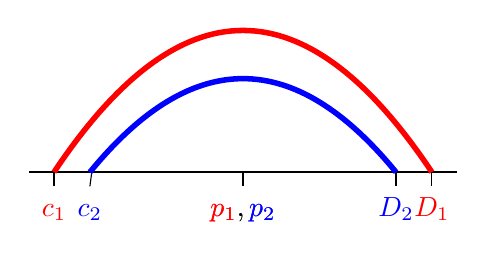
\begin{tikzpicture}[xscale=0.8, yscale=0.3]
% \draw [help lines,color=green]  (-7,-1) grid (7,7); 
%%%%%%%%%
\draw [thick] (-3.4,0) -- (3.4,0);
\coordinate (P0) at (0,6);
\coordinate (P1) at (1,6);
\coordinate (P2) at (2,4);
\coordinate (P3) at (3,0);
\draw [line width=2pt, red] (P0) .. controls (P1) and (P2) .. (P3);
\coordinate (P1) at (-1,6);
\coordinate (P2) at (-2,4);
\coordinate (P3) at (-3,0);
\draw [line width=2pt, red] (P0) .. controls (P1) and (P2) .. (P3);
\draw (0,0) -- (0,-.6) node [yshift=-.3cm] {{\strut$\R{p_1},\B{p_2}$}};
\draw (-3,0) -- (-3,-.6) node [yshift=-.3cm] {\R{\strut$c_1$}};
\draw (3,0) -- (3,-.6) node [yshift=-.3cm] {\R{\strut$D_1$}};
\draw (-2.4,0) -- (-2.43,-.6) node [yshift=-.3cm] {\B{\strut$c_2$}};
\draw (2.43,0) -- (2.43,-.6) node [yshift=-.3cm] {\B{\strut$D_2$}};
\draw (0,0) -- (0,-.6) node [yshift=-.3cm] {{\strut$\R{p_1},\B{p_2}$}};
\begin{scope}[xscale=.81, yscale=0.66] 
\coordinate (P0) at (0,6);
\coordinate (P1) at (1,6);
\coordinate (P2) at (2,4);
\coordinate (P3) at (3,0);
\draw [line width=2pt, blue] (P0) .. controls (P1) and (P2) .. (P3);
\coordinate (P1) at (-1,6);
\coordinate (P2) at (-2,4);
\coordinate (P3) at (-3,0);
\draw [line width=2pt, blue] (P0) .. controls (P1) and (P2) .. (P3);
\end{scope} 
\end{tikzpicture}
\vskip -23ex 

\pause
Optimal \7{myopic} price $p_i=(c_i+D_i)/2$.
~~~
\example

\qquad\R{$D_1=207$},
\B{$D_2=193$},
$\R{p_1}=\B{p_2}=132$,
profits $\R{75^2}$, $\B{61^2}$. 

\vpause
Played over 25 periods $t=1,\ldots,25$,

\qquad$\R{D_1^1}=\B{D_1^1}=200$

\qquad$\R{D_1^{t+1}=D_1^{t}+(\B{p_2^t}-p_1^t)/2}$

\qquad$\B{D_2^{t+1}=D_2^{t}+(\R{p_1^t}-p_2^t)/2}$

\end{frame}
%%%%%%%%%%%%%%%%%%%%%%%%%%%%%%%%%%%%%%%%% 
\begin{frame}
{Cooperative solution}

If both producers always choose myopic duopoly price:
\[
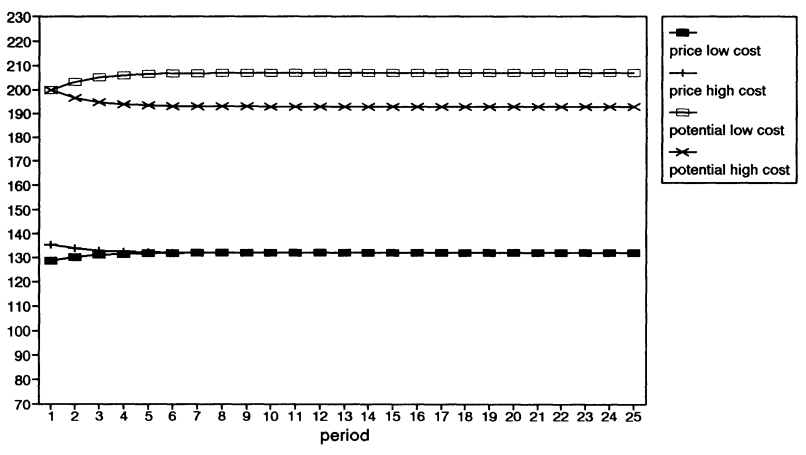
\includegraphics[width=.85\hsize]{myopic.png}
\]
Total profits over 25 periods about \R{$156$k}, \B{$109$k}

\end{frame}
%%%%%%%%%%%%%%%%%%%%%%%%%%%%%%%%%%%%%%%%% 
\begin{frame}
{Subgame perfect equilibrium}

Via parameterized backward induction:
\[
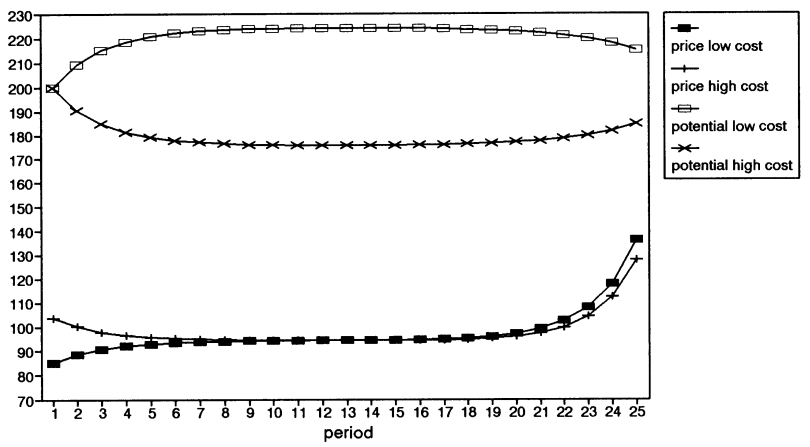
\includegraphics[width=.85\hsize]{spne.png}
\]
Total profits about \R{$137$k}, \B{$61$k}

\end{frame}
%%%%%%%%%%%%%%%%%%%%%%%%%%%%%%%%%%%%%%%%% 
\begin{frame}
{Strategy experiments}

\vskip1ex
Submitted strategy = flowchart pair, for
\R{low-cost} and \B{high-cost} 
firm.
% \\
% Competition rounds 1 (45 entries) and 2 (34) with feedback.

Two competition rounds:

first round: 45 entries

(after feedback:)
\\
second round: 34 entries

\strut

second-round profits:
\vskip-20ex

\strut\hfill
% 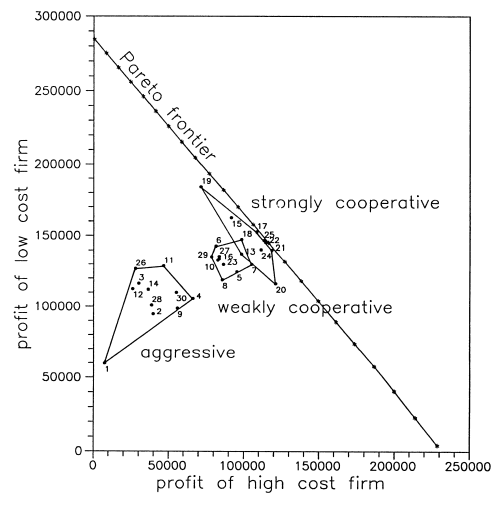
\includegraphics[width=.55\hsize]{pareto.png}
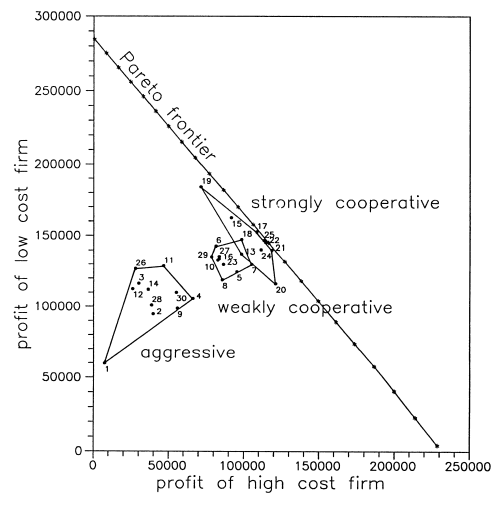
\includegraphics[width=.6\hsize]{pareto.png}

% \vskip-20ex

\end{frame}
%%%%%%%%%%%%%%%%%%%%%%%%%%%%%%%%%%%%%%%%% 
\begin{frame}
{Lessons from a participant's perspective}

\parskip1.5ex
Profits were totalled against all other teams (including own
type)

\0
\7{Very important for doing well:}~~ \B{understanding} the game
\8
focus on demand potential, not price
\8
smaller price \R{strongly} increases future profits
\8
avoid wild swings
\8
exploit ``suckers''

\pause
\0
No clear ``cooperative behavior''; myopic play is a focal
point

\pause
\0
Strategies \7{react} (typically to last price) but have
\7{no model of the opponent}
\8
one team reacted to \7{predicted} rather than past
behavior

\pause
\0
``Optimization'' of parameters typically against self-play.

\end{frame}
%%%%%%%%%%%%%%%%%%%%%%%%%%%%%%%%%%%%%%%%% 
\begin{frame}
{The learning framework}

\0
\B{Base game} = pricing game over 25 rounds, in two roles

\8
perhaps better: introduce \R{termination probability} of 4\%
after each round to \R{avoid end effect}, leads to random number of
rounds;
reward is then average profit per round

\pause
\0
\B{strategy} (\B{agent}) represented by a neural
network that chooses the \7{next price} as a function of
data for the last, say, $3$ periods 

\pause
\0
agent is \7{trained} by repeatedly meeting another
random agent, \7{drawn} from a \7{mixed equilibrium} of
existing strategies, which define the \R{population game}
of pairwise interactions
\pause

\0
a successfully trained strategy is \7{added} to the
population game
\8
new entrant has payoffs against each existing strategy
\8
defines a bimatrix game with new equilibrium as next
learning environment 

\end{frame}
%%%%%%%%%%%%%%%%%%%%%%%%%%%%%%%%%%%%%%%%% 
\begin{frame}
{\fbox{Learning a new strategy: issues}}

\7{Main assumption: }
the learning environment is \B{constant} (not evolving with the
learning agent) but \R{random} (mixed equilibrium)

\0
a whole strategy, for unknown situations, must be learned

\0
assumption: learn next price as \7{function} of last $3$ periods with
\8
information per period: \R{own price, own profit}, opponent price
\8
implicit \R{(or explicit?) \7{state}: demand potential} 
\pause
\0
\7{reward} function \5{\fbox{(critical: when?)}}\,: average per-period \R{profit} 
\pause
\0
for \B{population game}: profit recorded and updated \B{per opponent}
\8
weigh with length of interaction? (\ldots if less than 3
periods)? 
\0 how to initialize? vary an existing agent?
\0 when has an agent learned enough?

\end{frame}
%%%%%%%%%%%%%%%%%%%%%%%%%%%%%%%%%%%%%%%%% 
\begin{frame}
{A custom learning agent for this game}

Suppose the aim is a \7{strong strategy} for this game
(``feature engineering'', as in AlphaGo).

\parskip2ex
(Not for a general base game; use as benchmark?)

Tune a small set of \R{\7{parameters}} for a special own strategy:

\0 aim for a ``fair split'' of \R{demand potential}

\0 predict \R{opponent price} exponentially \R{$\alpha$-weighted}
from past
\8 in fact, opponent \R{sales} better predictor

\0 set own price to achieve target demand potential
\8 use \R{somewhat lower} price to steal customers

\end{frame}
%%%%%%%%%%%%%%%%%%%%%%%%%%%%%%%%%%%%%%%%% 
\begin{frame}
{The population game}

A successfully trained strategy is \7{added} to the
population game, as a \R{row} or \B{column}
depending on its role (\R{low-} or \B{high-cost} firm).
\8 (add only one row/column, or both?)

A new \7{equilibrium} is computed, typically \7{mixed}
and \7{not unique}.

That mixed equilibrium defines the next learning
environment.
\pause

\7{Which equilibrium?}
\0 \R{equilibrium selection} via computing an equilibrium from
random starting profile as \7{prior} (tracing procedure)
\8 as \7{proxy for \B{evolutionary dynamics}}
\8 finds only positive-index equilibria (for dynamic
stability)
\8 the prior could be the previous equilibrium
\0 has typically \B{small support} (no issue with PPAD-hardness)

\end{frame}
%%%%%%%%%%%%%%%%%%%%%%%%%%%%%%%%%%%%%%%%% 
\begin{frame}
{Index of a fixed point}

\[
\only<1>{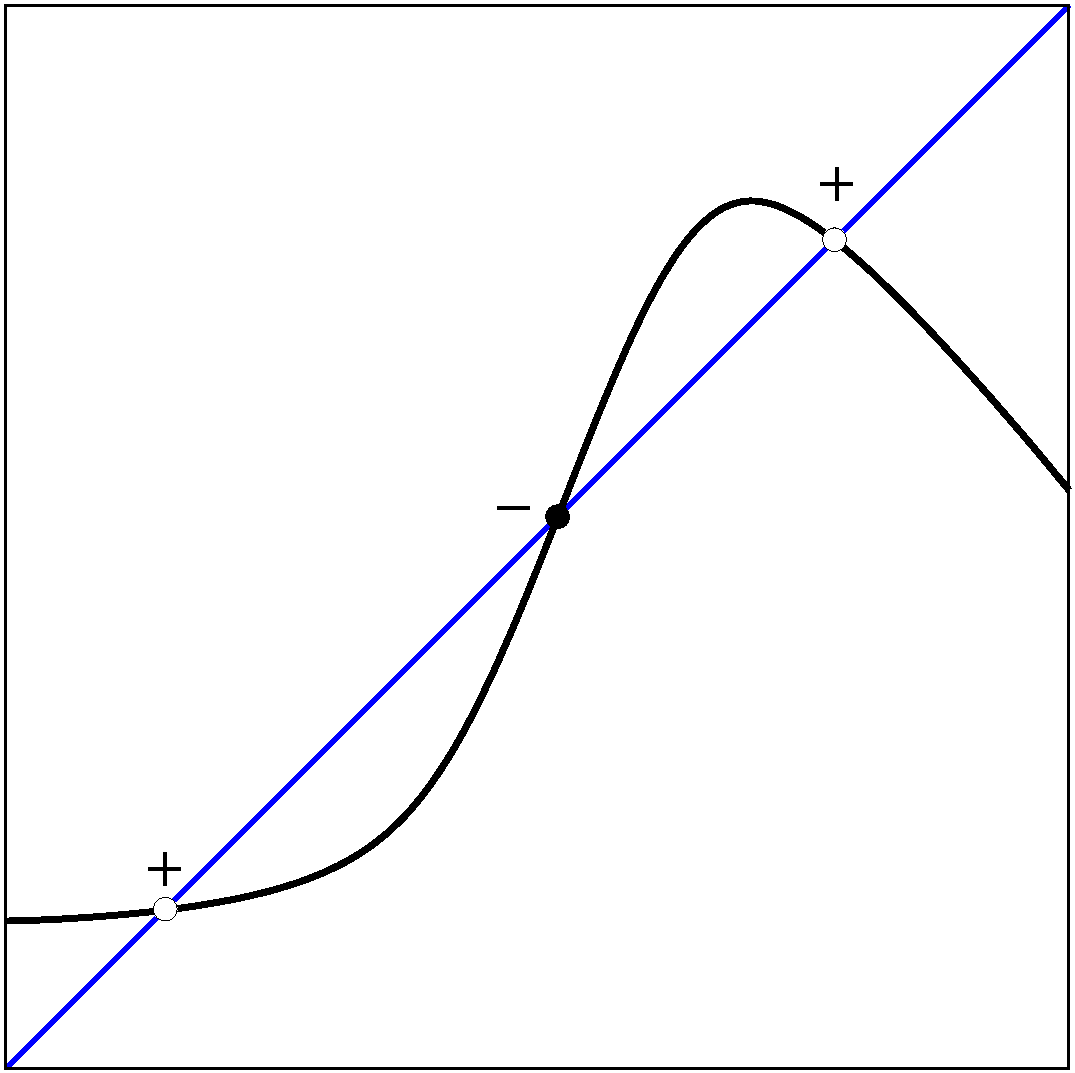
\includegraphics[height=60mm]{fixedonly.pdf}}
\only<2>{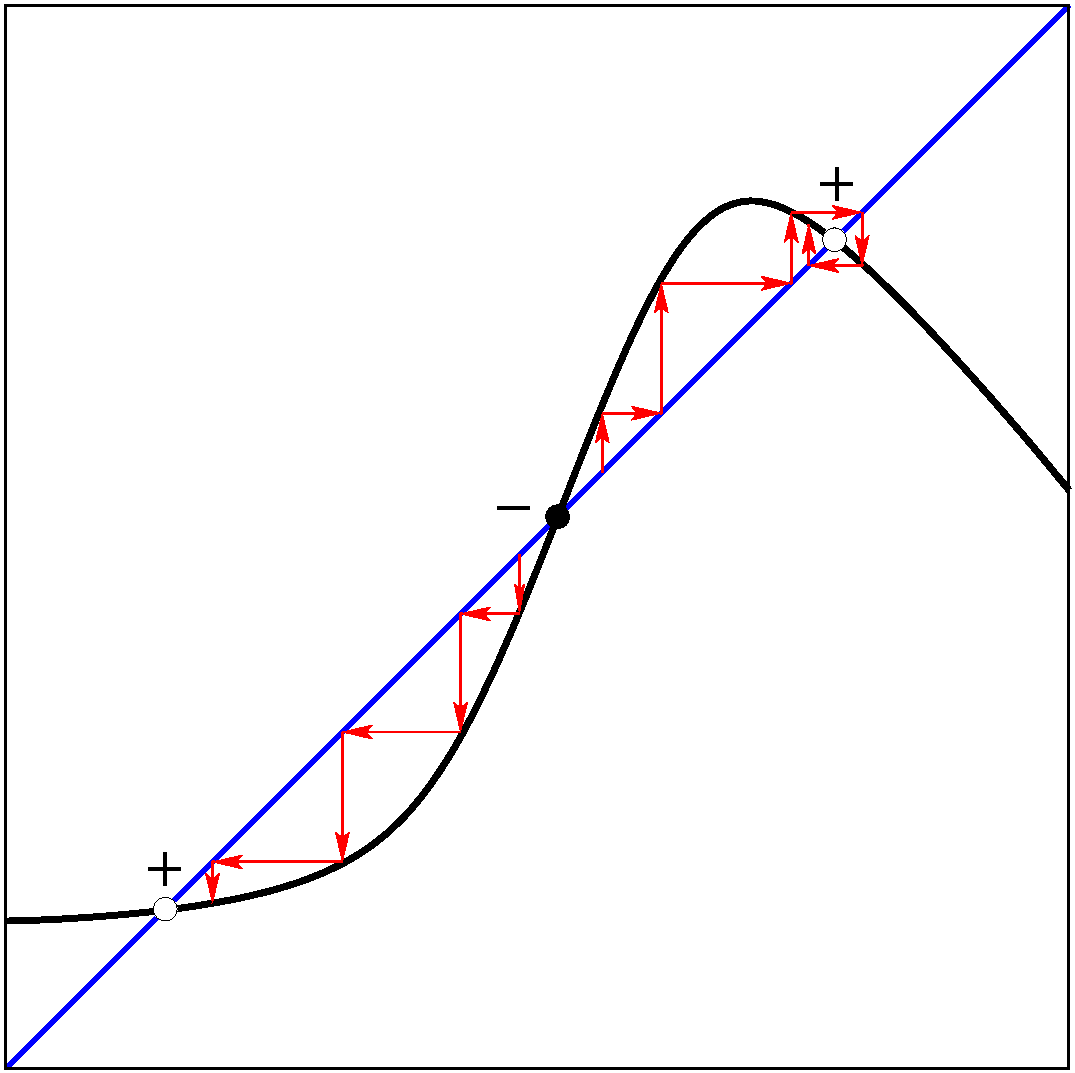
\includegraphics[height=60mm]{fixed.pdf}}
\]
Fixed point $x=f(x)$ :
% ~~~ index$(x)={}$sign det ($\B{Id}-D f(x)$)
~~~ index$(x)={}$sign det $D(\B{x}- f(x)$)

\onslide<2>{positive index necessary for \R{dynamic stability}}

\end{frame}
%%%%%%%%%%%%%%%%%%%%%%%%%%%%%%%%%%%%%%%%% 
\begin{frame}
{Example of a mixed equilibrium}

\vskip2ex
\renewcommand{\bimatrixrowcolor}{Red}
\renewcommand{\bimatrixcolumncolor}{Blue} 
\renewcommand{\7}{\fbox}
\[
\bimatrixgame{1em}{4}{4}{L}{H}%
{{$A$}{$B$}{$C$}{$D$}}%
{{$a$}{$b$}{$c$}{$d$}}
{
% \payoffpairs{1}{{$152$}{\fbox{$180$}}{$157$}{$154$}}{{\fbox{$100$}}{$86$}{$98$}{$99$}}
% \payoffpairs{2}{{$74$}{$170$}{\fbox{$178$}}{$130$}}{{\fbox{$110$}}{$66$}{$47$}{$75$}}
% \payoffpairs{3}{{\fbox{$155$}}{$160$}{$156$}{$157$}}{{$102$}{\fbox{$103$}}{\fbox{$103$}}{\fbox{$103$}}}
% \payoffpairs{4}{{$154$}{$158$}{$155$}{\fbox{$159$}}}{{\fbox{$105$}}{\fbox{$105$}}{\fbox{$105$}}{$104$}}
\payoffpairs{1}{{152}{\7{180}}{157}{154}}{{\7{100}}{86}{98}{99}}
\payoffpairs{2}{{74}{170}{\7{178}}{130}}{{\7{110}}{66}{47}{75}}
\payoffpairs{3}{{\7{155}}{160}{156}{157}}{{102}{\7{103}}{\7{103}}{\7{103}}}
\payoffpairs{4}{{154}{158}{155}{\7{159}}}{{\7{105}}{\7{105}}{\7{105}}{104}}
\pause
\put(17,-2){equilibrium}
\put(17,-3){payoffs:}
\R{%
\put(-4,-2){\mm{$0.02$}}
\put(-4,-6){\mm{$0.01$}}
\put(-4,-10){\mm{$0.67$}}
\put(-4,-14){\mm{$0.30$}}
\put(18,-7){\mm{$156$}}
}\B{%
\put(2,2.5){\mm{$0.05$}}
\put(6,2.5){\mm{$0.03$}}
\put(10,2.5){\mm{$0.58$}}
\put(14,2.5){\mm{$0.34$}}
\put(20,-5){\mm{$103$}}
}}
\]

\end{frame}
%%%%%%%%%%%%%%%%%%%%%%%%%%%%%%%%%%%%%%%%% 
\begin{frame}
{``Market share'' as different reward function?}

In a mixed equilibrium, all pure best responses have equal
payoff.

$\Rightarrow$ ~~~
mixed-strategy probabilities depend on \R{opponent} payoffs

\example Inspection game

\vskip-3ex

\strut\hskip17mm
{\small
\bimatrixgame{4.1mm}{2}{2}{}{}%
{{Don't inspect}{Inspect}}%
{{comply}{cheat}}%
{
\payoffpairs{1}{{\fbox{$0$}}{$-10$}}{{$0$}{\fbox{$10$}}}
\only<1>{\payoffpairs{2}{{$-1$}{\fbox{$-6$}}}{{\fbox{$0$}}{$-40$}}}
\only<2->{\payoffpairs{2}{{$-1$}{\fbox{$-6$}}}{{\fbox{$0$}}{$-90$}}}
\only<1>{\put(-2,-1){\mm{\strut\R{$0.8$}}}\put(-2,-5){\mm{\strut\R{$0.2$}}}}
\only<2->{\put(-2,-1){\mm{\strut\R{$0.9$}}}\put(-2,-5){\mm{\strut\R{$0.1$}}}}
% \pause
% \put(-6,-9.5){\mbox{\strut\B{expected payoffs:}}}%
% \put(2.7,-9.5){\mbox{\strut\B{$0$}}}%
% \put(5,-9.5){\mbox{\strut\B{$(1-p)10-90p$}}}%
% \put(5,-10.5){\mbox{\strut\B{${}=10-100p$}}}%
\put(2,2){\mm{\strut\B{$0.8$}}}%
\put(6,2){\mm{\strut\B{$0.2$}}}%
%
}\onslide<3->{\strut\hfill

\includegraphics[height=50mm]{parking.jpg}~~}}

\onslide<4>{Learn to \7{treat opponents
equally} to get high population share?}

\end{frame}
%%%%%%%%%%%%%%%%%%%%%%%%%%%%%%%%%%%%%%%%% 
\begin{frame}
{Advantage of this framework}

It is 
\7{modular} rather than a huge simulation:

\0
the \R{base game} (pricing game)
\8 is complex \5{(too complex?)} as an interesting learning scenario
\8 allows competition and cooperation
\8 potentially has ``hand-made'' good strategies
\8 can be replaced by another game

\0
the \B{population game} \ldots ~uses game theory
\8 provides via equilibria a ``stable'' learning environment
\8 has typically mixed, non-unique equilibria
\8 allows different equilibrium concepts (mixed, evolutionary)

$\Rightarrow$ ~~ 
%multiple ``comparative statics'' possible
can independently investigate different aspects

\end{frame}
%%%%%%%%%%%%%%%%%%%%%%%%%%%%%%%%%%%%%%%%% 
\begin{frame}
{Challenges ahead}

\0 ``Under control'': equilibrium computation for the
population game, tournament set-up

\0
\7{not yet:} implementing the learning agents

\0 comparison with existing approaches, e.g.
\linebreak
\REF{https://www.aeaweb.org/articles?id=10.1257/aer.20190623}{%
E. Calvano, G. Calzolari, V. Denicol\`o, and S. Pastorello
(2020), Artificial intelligence, algorithmic pricing, and
collusion.
\linebreak
\textit{American Economic Review} 110(10),
3267--3397.}

\vskip2ex
\5{\7{Future extension:}}

\0 competition between more than two firms (better model)

\0 different base games


\end{frame}
%%%%%%%%%%%%%%%%%%%%%%%%%%%%%%%%%%%%%%%%% 
\begin{frame}

\centering{\Huge Thank you!}

\end{frame}
%%%%%%%%%%%%%%%%%%%%%%%%%%%%%%%%%
\end{document}
